\chapter{Билет №10}

\section*{Создание собственной файловой системы. Структура, описывающая файловую систему и пример ее заполнения. Регистрация и дерегистрация файловых систем. Монтирование файловой системы. Структура \\struct super\_operations. \\ Структура inode\_operations. Функции simple и generic. Точка монтирования. Функции монтирования. Функция printk(). Пример создания файловой системы, ее регистрация и монтирование (лаб. раб.).}


\section{Файловая подсистема}
Файл --- важнейшее понятие в файловой подсистеме. Файл --- информация, хранимая во вторичной памяти или во вспомогательном ЗУ с целью ее сохранения после завершения отдельного задания или преодоления ограничений, связанных в объемом основного ЗУ.

Файл --- поименованная совокупность данных, хранимая во вторичной памяти (возможно даже целая). Файл --- каждая индивидуально идентифицированная единица информации.

Существует 2 ипостаси файла:
\begin{enumerate}
	\item файл, который лежит на диске;
	\item открытый файл (с которым работает процесс).
\end{enumerate}

Открытый файл --- файл, который открывает процесс.

Файл != место на диске. В мире современной вычислительной техники файлы имеют настолько большие размеры, что не могут храниться в непрерывном физическом адресном пространстве, они хранятся вразброс (несвязанное распределение).

Файл может занимать разные блоки/сектора/дорожки на диске аналогично тому, как память поделена на страницы. В любой фрейм может быть загружена новая страница, как и файл. 

Также, важно понимать адресацию. 

Соответственно, система должна обеспечить адресацию каждого такого участка.

\begin{quote}
	ОС является загружаемой программой, её не называют файлом, но когда компьютер включается, ОС находится во вторичной памяти. Затем с помощью нескольких команд, которые находятся в ПЗУ, ОС (программа) загружается в ОЗУ. При этом выполняется огромное количество действий, связанных с управлением памятью, и без ФС это сделать невозможно. Любая ОС без ФС не может быть полноценной.
\end{quote}

Задача ФС --- обеспечивать сохранение данных и доступ к сохраненным данным (обеспечивать работу с файлами).

Чтобы обеспечить хранение файла и последующий доступ к нему, файл должен быть изолирован, то есть занимать некоторое адресное пространство, и это адресное пространство должно быть защищено. Доступ обеспечивается по тому, как файл идентифицируется в системе (доступ осуществляется по его имени).

ФС --- порядок, определяющий способ организации хранения, именования и доступа к данным на вторичных носителях информации.

\begin{quote}
	File management (управление файлами) --- программные процессы, связанные с общим управлением файлами, то есть с размещением во вторичной памяти, контролем доступа к файлам, записью резервных копий, ведением справочников (directory).
	
	Основные функции управления файлами обычно возлагаются на ОС, а дополнительные --- на системы управления файлами.
	
	Доступ к файлам: open, read, write, rename, delete, remove.
	
	Разработка UNIX началась с ФС. Без ФС невозможно создание приложений, работающих в режиме пользователя (сложно разделить user mode и kernel mode).
	
	Файловая подсистема взаимодействует практически со всеми модулями ОС, предоставляя пользователю возможность долговременного хранения данных, а также ОС возможность работать с объектами ядра.
\end{quote}

\section{Особенности файловой подсистемы \\ Unix/Linux}
В Unix все файл, если что-то не файл, то это процесс.

В системе имеются спец. файлы, про которые говорят, что они больше чем файл: программмные каналы, сокеты, внешние устройства.

Файловая система работает с регулярными (обычными) файлами и директориями. При этом Unix/Linux не делают различий между файлами и директориями.

Директория -- файл, который содержит имена других файлов.

7 типов файлов в Unix:
\begin{enumerate}
    \item '-' -- обычный файл
    \item 'd' -- directory
    \item 'l' -- soft link
    \item 'c' -- special character device
    \item 'b' -- block device
    \item 's' -- socket
    \item 'p' -- named pipe
\end{enumerate}

\section{Иерархическая структура файловой подсистемы}

\begin{quote}
Существует стандарт FileSystem Hierarchy Standard (FHS), который определяет структуру и содержимое каталогов в Linux distribution (Ubuntu поддерживает этот стандарт).

По этому стандарту корень файловой системы обозначается как «/» (корневой каталог) и его ветви обязательно должны составлять единую файловую систему, расположенную на одном носителе (диске или дисковом разделе). В нем должны располагаться все компоненты, необходимые для старта системы.
\end{quote}

\begin{table}[h!]
  \centering
  \begin{tabular}{p{1\linewidth}}
    \centering
    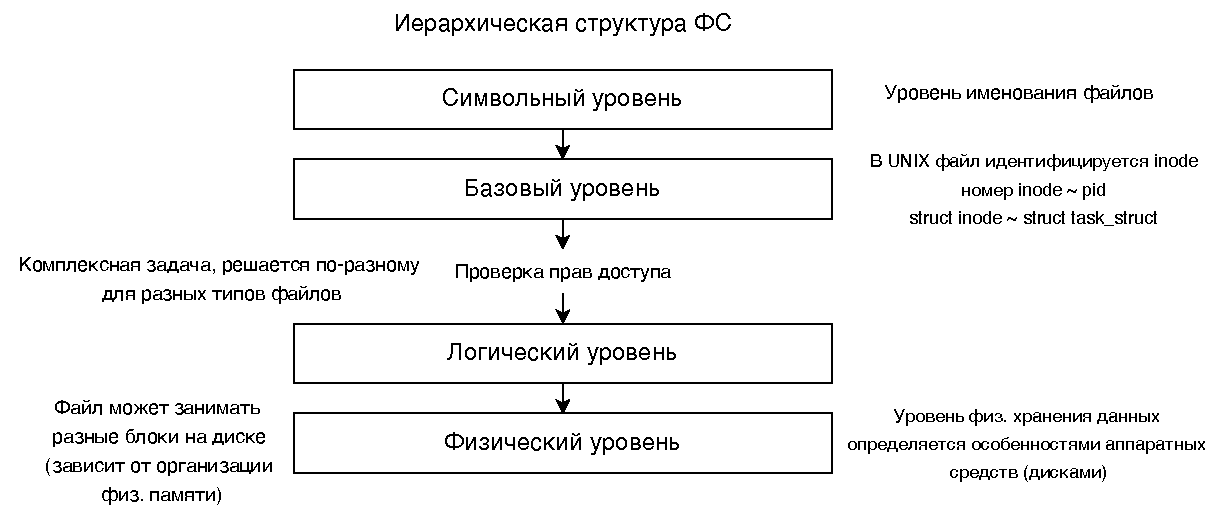
\includegraphics[width=0.8\linewidth]{./images/ierarh_fs.pdf}
  \end{tabular}
\end{table}

\begin{quote}
\textbf{Символьный уровень}

Это уровень именования файлов. Сюда входит организация каталогов, подкаталогов.

В Unix/Linux имя файла не является его идентификатором. Один и тот же файл может иметь множество имён (hard link). Это делалось для того, чтобы к одному и тому же файлу можно было получать доступ из разных директорий. Файлы в системе идентифицируются с помощью inode.

Символьный уровень — самый верхний уровень файловой системы, именно он связан с именованием файлов и позволяет пользователю работать с файлами (так как помнить inode своих файлов сложно).

\textbf{Базовый уровень}

Это уровень формирования дескриптора файлов. Должны быть соответствующие структуры, позволяющие хранить необходимую для файла информацию.

В ядре существует два типа inode (Index Node): дисковый и ядрёный. Чтобы получить доступ к файлу требуется перейти с символьного уровня к номеру inode, которым и идентифицируется в системе файл.

Обоснованием использования двух типов inode в системе является факт того, что Unix изначально создавалась как система которая поддерживает очень большие файлы. Для того чтобы адресовать данные которые находятся в этих файлах, необходимо иметь соответствующие структуры. Так как именно inode как сейчас принято говорить, является дескриптором файла, то такая информация должна храниться в дисковом inode.

\textbf{Логический уровень}

Логическое адресное пространство файла аналогично адресному пространству процесса: оно начинается с нулевого адреса и представляет собой непрерывную последовательность адресов. Непрерывное адресное пространство, начинающееся с 0.

\textbf{Физический уровень}

Это уровень хранения и доступа к данным.

\end{quote}

\section{Создание собственной файловой системы}

Чтобы создать собственую ф.с. В struct superblock есть поле file\_system\_type (структура ядра)

После описания ф.с., ядро предоставляет возможность зарегистрировать/удалить ф.с.

Структура описывающая конкретный тип ф.с. может быть только 1. При этом одна и та же ф.с. мб подмонтирована много раз.

Пример создания собств. ф.с.

Инициализация полей структуры \\ file\_system\_type
\begin{lstlisting}
	struct file_system_type fs_type =
	{
		.owner = THIS_MODULE,
		.name = "myfs",
		.mount = myfs_mount,
		.kill_sb = kill_litter_super
	}
\end{lstlisting}

В функции myfs\_mount можно вызвать mount\_bdev/ mount\_nodef/ \\ mount\_single

При создании ФС мы инициализируем лишь следующие поля:

\begin{itemize}[label=---]
	\item owner - нужно для организации счетчика ссылок на модуль (нужен, чтобы система не была выгружена, когда фс примонтирована).
	\item name - имя ФС.
	\item  mount - указатель на функцию, которая будет вызвана при монтировании ФС.
	\item kill\_sb - указатель на функцию, которая будет вызвана при размонтировании ФС.
\end{itemize}

Разработчик ф.с. должен определить набор функций для работы с файлами в своей ф.с. Для этого используется struct file\_operations.

\section{Регистрация и дерегистрация файловой системы}

Для регистрации ф.с. ядро предоставляет ф-цию register\_filesystem() (для удаления unregister\_filesystem). Функции \\ register\_filesystem передается инициализированная структура file\_system\_type.


\section{Монтирование файловой системы. Точка монтирования}

Фактически VFS — интерфейс, с помощью которого ОС может работать с большим количеством файловых систем.

Основной такой работы (базовым действием) является монтирование: прежде чем файловая система станет доступна (мы сможем увидеть ее каталоги и файлы) она должна быть смонтирована.

Монтирование — подготовка раздела диска к использованию файловой системы. Для этого в начале раздела диска выделяется структура super\_block, одним из полей которой является список inode, с помощью которого можно получить доступ к любому файлу файловой системы.

Когда файловая система монтируется, заполняются поля struct vfsmount, которая представляет конкретный экземпляр файловой системы, или, иными словами, точку монтирования. Точкой монтирования является директория дерева каталогов.

Вся файловая система должна занимать либо диск, либо раздел диска и начинаться с корневого каталога.

Любая файловая система монтируется к общему дереву каталогов (монтируется в поддиректорию).

И эта подмонтированная файловая система описывается суперблоком и должна занимать некоторый раздел жесткого диска ("это делается в процессе монтирования").

Когда файловая система монтируется, заполняются поля структуры super\_block.

super\_block содержит информацию, необходимую для монтирования и управления файловой системой.

\begin{quote}
	Пример: мы хотим посмотреть содержимое флешки. Флешка имеет свою файловую систему, она может быть подмонтирована к дереву каталогов, и ее директории, поддиректории и файлы, которые мы сохраним на флешке, будут доступны. Потом мы достаем флешку. "Хорошая" система контролирует это и сделает демонтирование файловой системы за нас.
\end{quote}

\begin{quote}
	Если в системе присутствует некоторый образ диска image, а также создан каталог, который будет являться точкой монтирования файловой системы dir, то подмонтировать файловую систему можно, используя команду: mount -o loop -t myfs ./image ./dir
	
	Параметр -o указывает список параметров, разделенных запятыми. Одним из прогрессивных типов монтирования, является монтирование через петлевое (loop, по сути, это «псевдоустройство» (то есть устройство, которое физически не существует --- виртуальное блочное устройство), которое позволяет обрабатывать файл как блочное устройство) устройство. Если петлевое устройство явно не указано в строке (а как раз параметр -o loop это задает), тогда mount попытается найти неиспользуемое в настоящий момент петлевое устройство и применить его.
	
	Аргумент следующий за -t указывает тип файловой системы.
	
	./image - это устройство. ./dir - это каталог.
	
	umount — команда для размонтирования файловой системы:
	
	umount ./dir
\end{quote}

\section{Раздел жесткого диска и super\_block}
\par Если пользователь желает, чтобы фс стала доступна (пользователь сможет получить доступ к файлам и каталогам данной фс), она должна быть подмонтирована и для нее должен быть выделен раздел жесткого диска.
\par Раздел на диске -- выделенное адресное пространство.
\par первая структура в разделе -- superblock.

\begin{table}[h!]
  \centering
  \begin{tabular}{p{1\linewidth}}
    \centering
    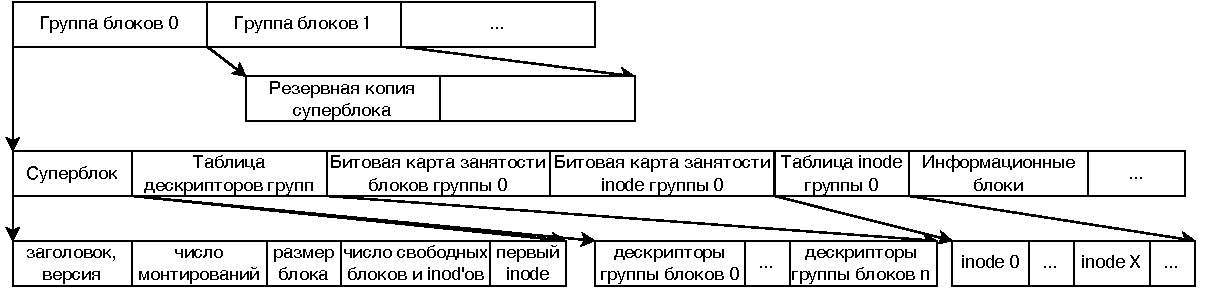
\includegraphics[width=1\linewidth]{./images/partition.pdf}
  \end{tabular}
\end{table}

\par Размер блока (на диске) -- непрерывное адресное пространство. В современных вычислительных система файлы относительно большие, поэтому она не могут храниться в непрерывном адресном пространстве. Она хранятся вразброс в свободных блоках. Система должна иметь возможность обращаться к каждому блоку, в котором хранится информация. Для этого в inode имеются соответствующие ссылки.
\par Чтобы система могла мобильно выделять файлам новые блоки, необходимо иметь соответствующую информацию.
\par \textbf{s\_blocksize} -- имя поля в \textbf{struct \\ super\_block}
\par Первый inode -- inode корневого каталога фс.

В группе блоков 1 находится резервная копия суперблока. В каждой фс один super\_block, и он располагается в начале раздела. У него есть копия для обеспечения надежности работы с фс, хранения файлов, super\_block считывается в память ядра при монтировании фс и находится там до ее демонтирования (или завершения работы с системой).

timestamps -- временные отметки, указывающие время модификации inode: 
\begin{itemize}
\item ctime -- время модификации inode
\item mtime -- время модификации файла
\item atime -- время последнего доступа к файлу.
\end{itemize}

Блок может быть адресован, следовательно мы знаем его адрес.

Битовая карта блоков (block bit map) -- структура, в которой каждый бит показывает, занят блок или нет (отведен ли он какому-то файлу)

Битовая карта inode -- выполняет аналогичную роль по отношению к таблице inod'ов. То есть показывает, какие индексные дескрипторы заняты, а какие свободны.

\section{Структура struct \\ super\_operations}
На любой структуре, лписывающей объект ядра, определены функции для работы с объектом соответсвующим типа (struct file\_operations, struct \\ inode\_operations, struct dentry\_operations).

\begin{lstlisting}
	struct super_operations {
		struct inode *(*alloc_inode)(struct super_block *sb);
		void (*destroy_inode)(struct inode *);
		
		void (*dirty_inode) (struct inode *, int flags);
		int (*write_inode) (struct inode *, struct writeback_control *wbc);
		int (*drop_inode) (struct inode *);
		void (*put_super) (struct super_block *);
		...
	};
\end{lstlisting}

dirty\_inode вызывается VFS, когда в индекс inode вносятся изменения (функция используется для изменения соотв таблицы структуры).

Ядро хранит копию таблицы inode-ов в памяти ядра, т.е. inode, к которому были обращения, кешируются для ускорения доступа к файлам. Сначала изменения вносятся в таблицу, к-ая находится в оперативной памяти.

Функция dirty\_inode позволяет отметить, что inode был изменен, и эту информацию надо скопировать в таблицу на диске.

write\_inode предназначена для записи inode на диск и помечает inode как измененный

put\_super вызывается VFS при размонтировании фс.


\section{Структура \\ inode\_operations}
Функции, определенные для работы с inode:
\begin{lstlisting}
	struct inode_operations {
		struct dentry * (*lookup) (struct inode *,struct dentry *, unsigned int);
		
		int (*create) (struct inode *,struct dentry *,
		umode_t, bool);
		
		int (*mkdir) (struct inode *,struct dentry *,
		umode_t);
		
		int (*rename) ( struct inode *, struct dentry *,
		struct inode *, struct dentry *, unsigned int);
		...
	} ;
\end{lstlisting}

Для поиска inode требуется, чтобы VFS вызывала функцию lookup() родительского каталога inode. Этот метод устанавливается конкретной реализацией файловой системы, в которой находится inode. Как только VFS находит требуемый dentry (и, следовательно, inode), можно открывать файл системным вызовом open или получать информацию о файле функцией stat, которая просматривает данные inode и передает часть их в пространство пользователя.


\section{Функции simple и generic}
Функции generic - заглушки.
\begin{lstlisting}
	int generic_delete_inode(struct inode *inode)
	{
		return 1;
	}
\end{lstlisting}

А функции simple выполняют некоторую простую последовательность действий, что освобождает разработчика от необходимости реализации этих действий каждый раз при реализации ФС. 
\begin{lstlisting}
	int simple_statfs(struct dentry *dentry, struct kstatfs *buf)
	{
		buf->f_type = dentry->d_sb->s_magic;
		buf->f_bsize = PAGE_CACHE_SIZE;
		buf->f_namelen = NAME_MAX;
		return 0;
	}
\end{lstlisting}


\section{Функция printk()}
Функция printk() определена в ядре Linux и доступна модулям. Функция аналогична библиотечной функции printf(). Загружаемый модуль ядра не может вызывать обычные библиотечные функции, поэтому ядро предоставляет модулю функцию printk(). Функция пишет сообщения в системный лог. Загрузка модулей в свою очередь выполнялась в пространстве ядра, где нет и не может быть никакого управляющего терминала, поэтому вывод printk() направляется демону системного журналирования, который помещает его, в частности, в системный журнал (/var/log/messages).

\section{Пример создания файловой системы, ее регистрация и монтирование (лаб. раб.)}
\begin{lstlisting}
	static struct dentry *my_vfs_mount(struct file_system_type *type, int flags, const char *dev, void *data)
	{
		// my_vfs_fill_sb - указатель на функцию, которая будет вызвана из mount_nodev для заполнения полей struct super_block
		// nodev - не различает файловые системы символьно-специальных и блочно-специальных устройств
		struct dentry *const root_dentry = mount_nodev(type, flags, data, my_vfs_fill_sb);
		    if (IS_ERR(root_dentry))
		printk(KERN_ERR "+ can't mount_nodev\n");
		else
		printk(KERN_INFO "+ VFS has been mounted.\n");
		
		return root_dentry;
		}
		
		static struct file_system_type my_vfs_type = {
		.owner = THIS_MODULE,
		.name = "myvfs",
		.mount = my_vfs_mount,
		.kill_sb = my_kill_super,
		};
		
		static int __init my_vfs_init(void){
		int rc = register_filesystem(&my_vfs_type);
		// ...
		return 0;
		}
		
		static void __exit my_vfs_exit(void)
		{
		// ...
		int rc = unregister_filesystem(&my_vfs_type);
		// error handling
		}
		
		module_init(my_vfs_init);
		module_exit(my_vfs_exit);
	\end{lstlisting}
	
\section*{Загадки}

Подмонтированные файловые системы через proc -> /proc/mounts

Зарегистрированные файловые системы через proc -> /proc/filesystems

Loop --- виртуальное блочное устройство (драйвер диска, который пишет данные не на физическое устройство, а в файл (образ диска))

Что означает nodev --- для монтирования не требуется блочное устройство

Какой минимальный набор действий для того, чтобы зарегистрировать собственную ФС? --- заполнить поле name в struct file\_system\_type и зарегистрировать функцией ядра register\_filesystem
    
Какой минимальный набор действий для того, чтобы можно было смонтировать
   собственную ФС? --- заполнить поля mount и name. Мы используем функция ядра mount\_nodev. Для функции mount мы должны передать функцию fill\_sb, которая будет заполнять superblock нашей ФС.
   
Если не указать оунера, то можно выгрузить модуль, не отмонтировав ФС, он считает количество монтирований (ссылок на модуль).

Для размонтирования обязательно указать нейм и килл суперблок.
   
Что за структура superblock, для чего нужна? --- описывает ПОДМОНТИРОВАННУЮ файловую систему.

Что нужно сделать внутри fill\_sb? Просто заполнить superblock же недостаточно? --- функция fill\_sb должна вернуть dentry КОРНЕВОГО каталога -> необходимо создать и проинициализировать dentry (d\_make\_root) -> необходимо создать и проинициализировать inode

Какой функцией создаете inode? --- new\_inode

Почему blocksize = PAGE\_SIZE? --- VFS расположена в оперативной памяти -> выделение оперативной памяти производится страницами

Слаб-кэш --- это высокопроизводительный аллокатор памяти, используемый в для ускорения доступа к файлу и для повторного использования проинициализированных слабов (брусков --- брусок характеризуется фиксированным размером) (их не придется заново инициализировать)

Создали свою структуру для инода, так как кэш под системный инод создается автоматически.
 
Зачем на каждый дентри там нужен айнод? --- ДЕНТРИ СОЗДАЕТСЯ НА ОСНОВЕ АЙНОДА: для долговременного хранения файла нужен айнод, так как он описывает физический файл, а дентри создается для айнода и нигде не хранится --- информация о папках хранится на диске, директория — это тоже файл, специального типа d. А поскольку это файл, ему нужен айнод. Айнод содержит информацию об адресах блоков, в которых хранится информация. В случае директории это информация о других файлах (тут можно нарисовать пример с /usr/ast/mbox). --- dentry существуют только в оперативной памяти, поэтому при выключении системы информация об элементах пути, если не хранить ее в виде файлов на диске (энергонезависимой части памяти), будет утеряна.

Что такое стракт айнод? --- дескриптор физического файла

Что такое монтирование? --- это выделение раздела диска под ФС, заполнение полей суперблока и помещение его в начало выделенного раздела. В суперблоке хранится массив айнодов, с помощью которого получаем доступ ко всем файлам ФС.

Основное действие при монтировании? --- это выделение раздела диска под ФС


